
Uloshyppypaikka määritetään laskemalla yhteen ajautuma varjon varassa sekä ajautuma vapaapudotuksessa. Näiden avulla saadaan selville sijainti ylätuulen puolella. Tämän paikan päällä lentokoneesta poistuva hyppääjä pääsee kaikkein varmimmin laskeutumisalueelle. Uloshyppypaikka ja hyppylinja määritetään aina toiminnan alkaessa. Jos epäillään olosuhteiden muuttuneen, on uloshyppypaikka määritettävä uudelleen. 


Peruskoulutukseen kuuluu vähintään viisi itsenäistä uloshyppypaikan määritystä. Laskeutumisen on tapahduttava kouluttajan määräämälle alueelle. 


Tässä luvussa annetaan ohjeellisia lukuja, joita voidaan käyttää UH-paikan määritykseen. Hyppääjät käyttävät kuitenkin hyvin vaihtelevaa varjokalustoa, ja paikanmääritykseen käytettyjen tuuliennusteiden tarkkuus vaihtelee. Arvioitua UH-paikkaa onkin syytä korjata jos hypättäessä osoittautuu, että laskeutumisalueelle on hankala päästä. 


Myös maassaolijat voivat tehdä näköhavaintoja esimerkiksi koneen sortamisesta hyppylinjalla. Näiden havaintojen avulla he voivat päättää oman uloshyppypaikkansa. Lisäksi kannattaa tarkkailla, missä hyppääjien varjot aukeavat maatuuleen nähden ja pääsevätkö hyppääjät helposti laskeutumisalueelle. Ajautuman arvioinnin tärkeys korostuu, jos laskeutumisalue on pieni, ilmassa on paljon muuta liikennettä tai tuuli on kova. 

\section{ Ajautuminen tuulen mukana }
\label{uloshyppypaikan-maaritys-ajautuminen-tuulen-mukana}


Vapaapudotuksen ja varjon ohjailun aikana tapahtuvan ajautumisen laskeminen on mahdollista, jos tunnetaan tuulet eri kerroksissa maanpinnan ja hyppykorkeuden välillä (ajautuma = tuulen nopeus m/s * pudottu aika s). Ylätuulet voidaan selvittää kysymällä tuulitiedot lentosääasemalta tai katsomalla ennusteista. Lisäksi tuulitietoja eri korkeuksista voidaan saada lentäjältä, mikäli lentokoneessa on GPS-laite. Tuulitietojen perusteella voidaan laskea ajautuman matka ja suunta tai arvioida ne riittävällä tarkkuudella. Tuulitietojen lisäksi on arvioitava eri ilmakerroksissa vietetty aika: 

\begin{itemize}
\item  Vapaapudotuksen ajaksi arvioidaan 50 sekuntia. 
\item  Hyppääjä vajoaa varjon varassa keskimäärin 5 m/s. 
\item  Varjon voidaan odottaa olevan täysin lentävä 800–1000 metrin korkeudessa. 
\item  Varjon varassa vietetyksi ajaksi saadaan siis noin 3 minuuttia. (180 s) 
\end{itemize}

Seuraavaan taulukkoon on laskettu yllä olevilla oletuksilla (lähimpään sataan metriin pyöristettyjä) ajautumia varjon varassa ja vapaapudotuksessa erilaisissa tuulissa. 

\begin{tabular}[]{|l|p{2.4cm}|l|}
\hline
 \textbf{tuuli (kt)} &  \textbf{varjon varassa (m)} &  \textbf{vapaassa (m)}
\\ \hline
 5 &  500 &  100
\\ \hline
 10 &  900 &  300
\\ \hline
 15 &  1400 &  400
\\ \hline
 20 &  1900 &  500
\\ \hline
 25 &  2300 &  600
\\ \hline
 30 &  2800 &  800
\\ \hline
 35 &  3200 &  900
\\ \hline
\end{tabular}
\subsection{ Ajautuminen varjon varassa }
\label{uloshyppypaikan-maaritys-ajautuminen-varjon-varassa}


Varjon varassa tapahtuvan ajautumisen laskemiseksi tarvitaan sekä avauskorkeuden että maatuulen tuulitiedot: nopeus ja suunta. Maatuuli voidaan myös jättää huomiotta ja käyttää vain tuulen nopeutta ja suuntaa esimerkiksi korkeuksissa 1000 ft ja 2000 ft. Tuulen suunnasta ja nopeudesta eri pinnoilla voidaan ottaa keskiarvot. 


Esimerkki ajautuman laskemisesta: 

\begin{tabular}[]{|l|r|r|}
\hline
 \textbf{Korkeus (ft)} &  \textbf{Suunta} &  \textbf{Nopeus (kt)}
\\ \hline
 2000 &  250 &  10
\\ \hline
 Pinta &  230 &  5
\\ \hline
 \textit{Keskiarvo} &  \textit{240} &  \textit{7,5}
\\ \hline
\end{tabular}

Ajautumaksi varjon varassa saadaan 700 metriä. Avauspaikka on siis 0,7 kilometrin etäisyydellä laskeutumisalueelta suuntaan 240 astetta. 

\subsection{ Ajautuminen vapaapudotuksessa }
\label{uloshyppypaikan-maaritys-ajautuminen-vapaapudotuksessa}


Vapaapudotuksessa tapahtuvan ajautumisen laskemiseen käytetään tuulitietoja avauskorkeuden ja uloshyppykorkeuden välillä.  


Esimerkki vapaapudotuksen ajautuman laskemiseen. 

\begin{tabular}[]{|l|r|r|}
\hline
 \textbf{Korkeus (ft)} &  \textbf{Suunta} &  \textbf{Nopeus (kt)}
\\ \hline
 12000 &  290 &  20
\\ \hline
 9000 &  270 &  15
\\ \hline
 6000 &  260 &  15
\\ \hline
 3000 &  250  &  10
\\ \hline
 \textit{Keskiarvo} &  \textit{270} &  \textit{15}
\\ \hline
\end{tabular}

Ajautumaksi vapaassa saadaan 400 metriä. Uloshyppypaikka sijaitsee siis 0,4 kilometriä avauspaikasta suuntaan 270. 


Uloshyppypaikka valitaan ajautuman verran tuulen yläpuolelta laskeutumisalueeseen nähden. Lentäjälle ja muille hyppääjille näytetään paikka koneessa olevalta kartalta tai kerrotaan paikka sanallisesti. 


\begin{Figure}\centering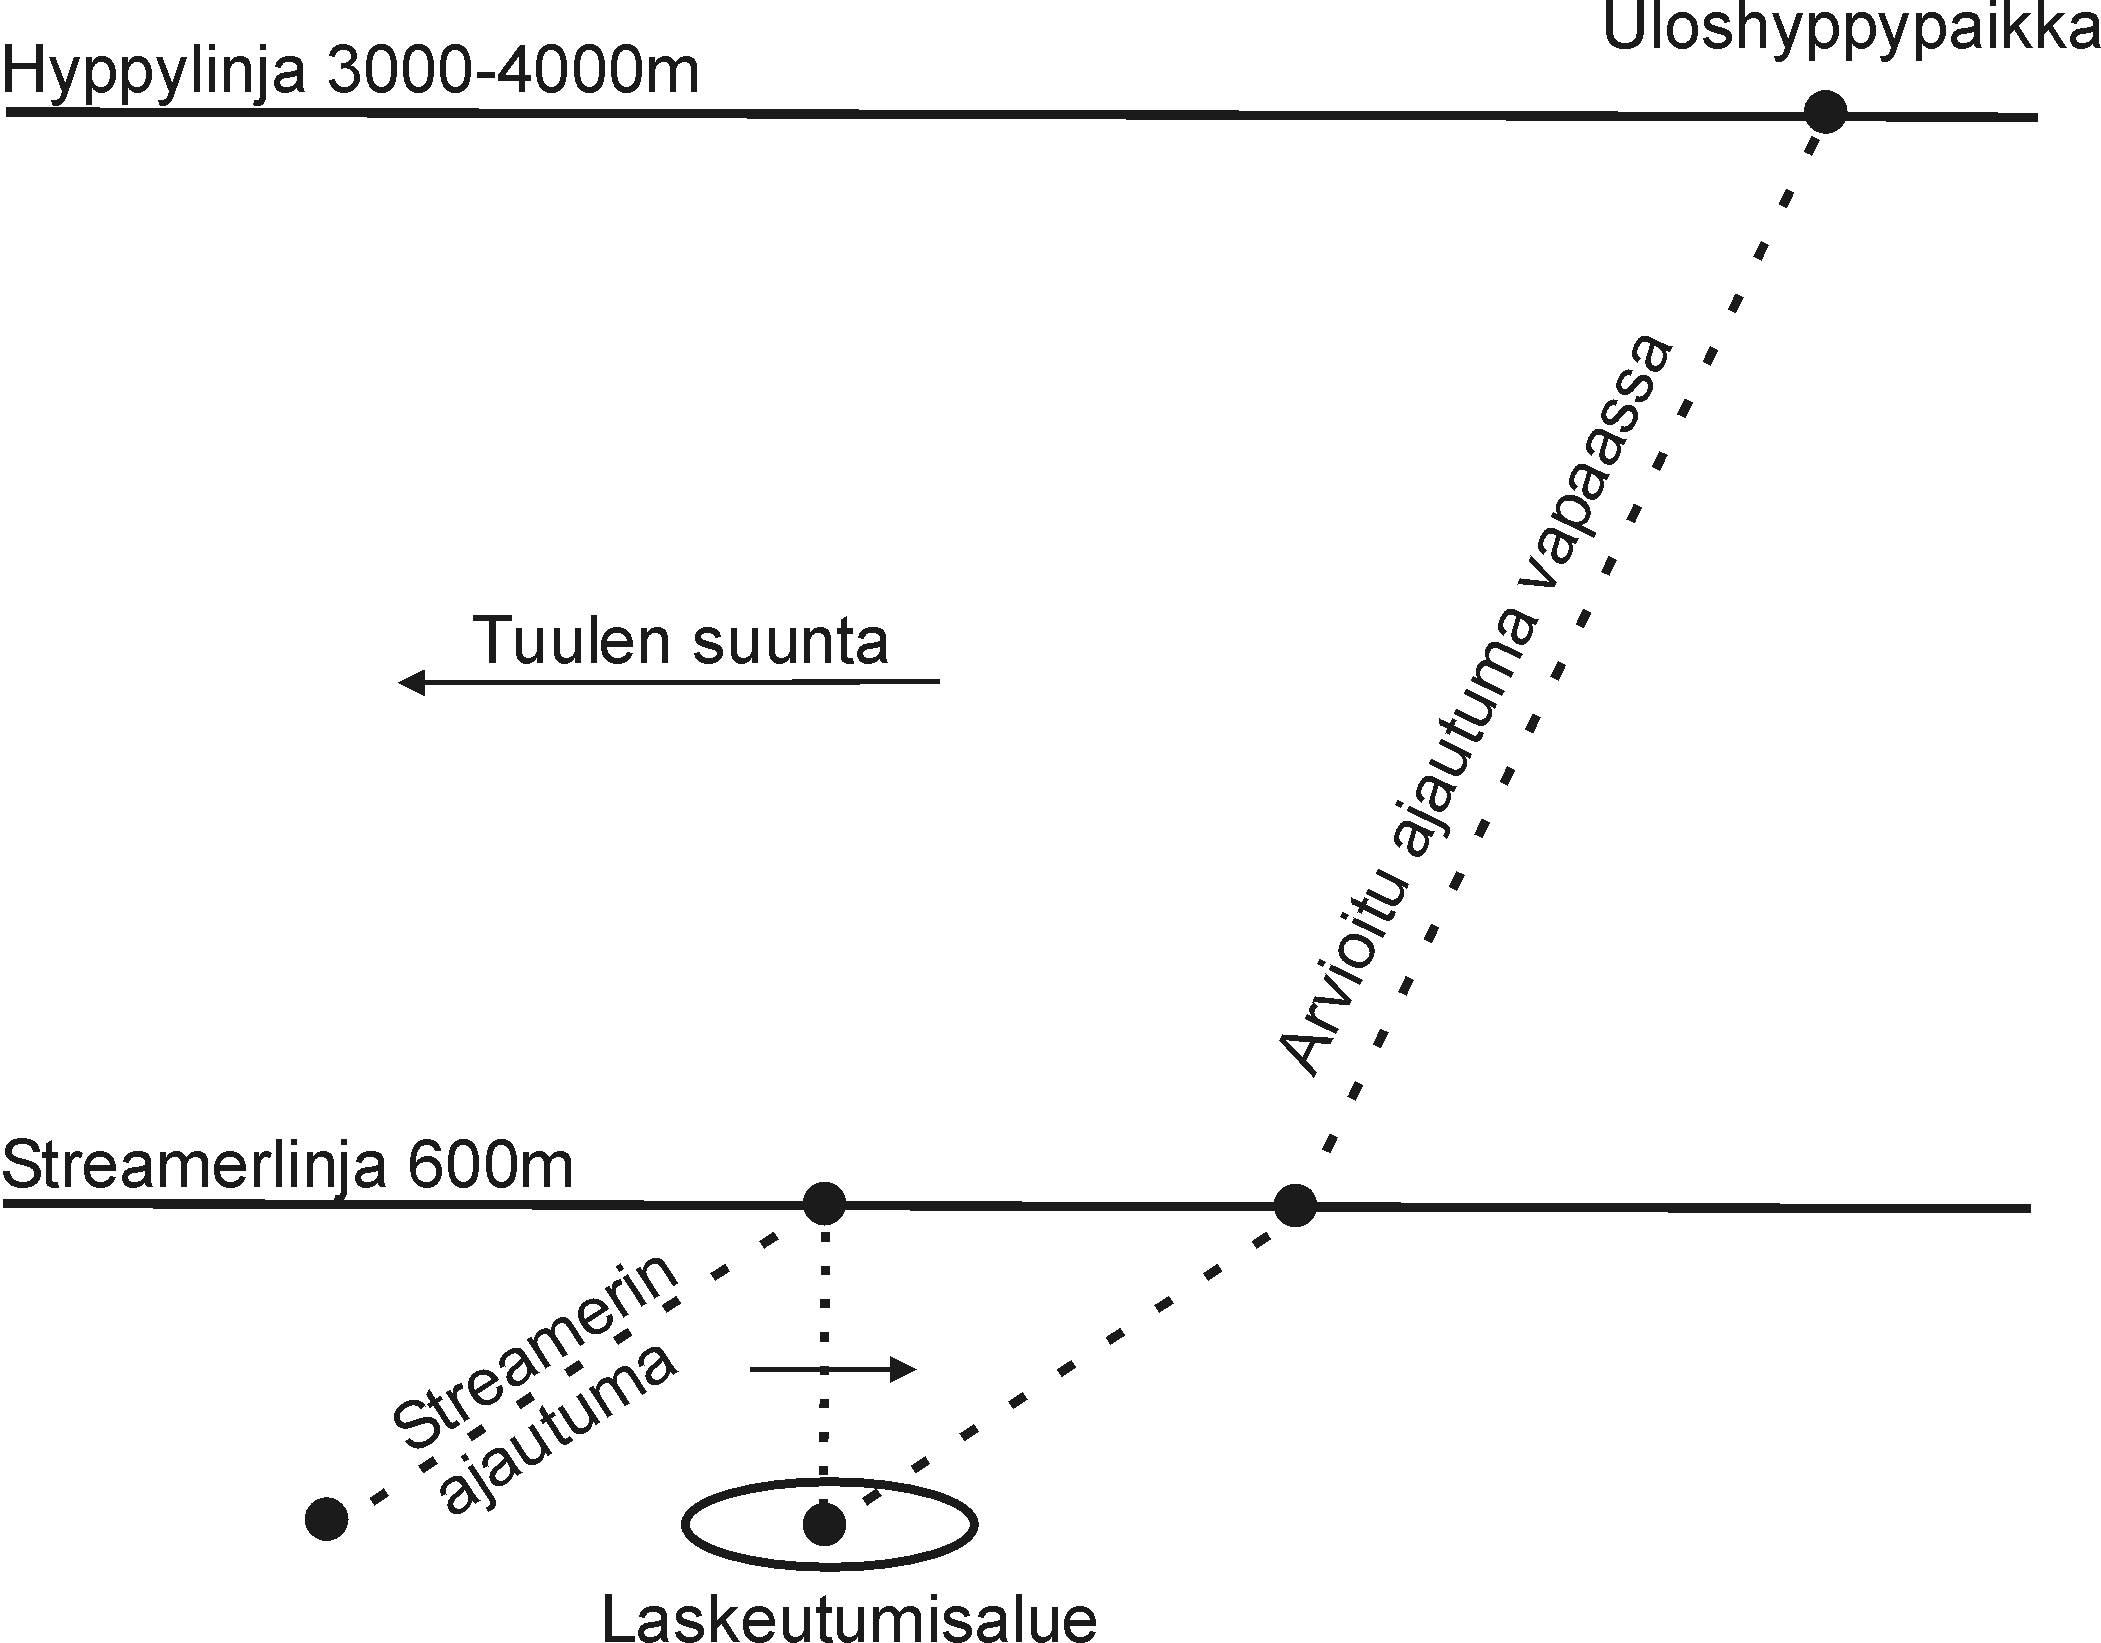
\includegraphics[width=0.99\textwidth]{Paikanmaaritys.jpeg}\captionof{figure}{Uloshyppypaikan määrittäminen korkeammalta hypättäessä}\end{Figure} 

\section{ Linjan määritys }
\label{uloshyppypaikan-maaritys-linjan-maaritys}


Jos lentokoneessa on useampia hyppääjiä/ryhmiä, määritetään hyppylinja huomioiden, että: 

\begin{itemize}
\item  Linja kulkee lasketun UH-paikan läpi. 
\item  Ryhmien välille tulee jäädä turvallinen välimatka. 
\item  Kaikkien tulee päästä turvallisesti laskeutumisalueelle. 
\end{itemize}

Pienillä hyppykoneilla linja ajetaan yleensä vastatuuleen laskeutumisalueen yli. Suurilla hyppykoneilla ajetaan usein sivutuulilinja tai esimerkiksi aina kiitotien suuntainen hyppylinja, jonka etäisyys laskeutumisalueesta riippuu tuuliolosuhteista. Linja voidaan ajaa tarvittaessa myös myötätuuleen. 


Linjan pituudelle ei ole yhtä oikeaa lukua, mutta sitä voidaan arvioida esim. seuraavasti. 

\begin{description}
\item[ ] \hfill \\ 
\textit{Laskuvarjon liitosuhde on välillä 3:1 ja 2:1. Jos hyppääjän varjo on auki 800 metrin korkeudessa ja hyppääjä aloittaa laskeutumiskuvion 300 metrin korkeudessa, hyppääjä voi lentää varjolla arviolta (500 m * 2,5) n. 1300 metrin matkan.}  \hfill \\ 
\end{description}

Tämän varsin konservatiivisen esimerkin mukaan linjan ensimmäinen ryhmä voisi siis poistua koneesta 1300 metriä ennen määritettyä UH-paikkaa ja viimeinen ryhmä 1300 metriä määritetyn pisteen jälkeen. Todellisuudessa linjan pituus voi vaihdella linjan suunnan, laskeutumisalueen, avauskorkeuksien jne. mukaan. Mitä kauempana oikeasta UH-paikasta hypätään, sitä suurempi on riski, että epätarkka tuuliennuste, sääolosuhteiden muutos, matala avaus tai varavarjon käyttö johtaa hyppääjän laskeutumiseen laskeutumisalueen ulkopuolelle. 

\section{Hyppääminen määritetyssä paikassa}
\label{uloshyppypaikan-maaritys-hyppaaminen-maaritetyssa-paikassa}


Lentäjälle annetaan ohjeet suunnitellusta paikasta ja lentosuunnasta ennen koneeseen nousua. Kun kone on saavuttanut hyppykorkeuden, lentäjä ohjaa sovitulle linjalle. Hyppylinja alkaa jo ennen laskeutumisaluetta.  

\subsubsection{Ohjeet lentäjälle}
\label{uloshyppypaikan-maaritys-ohjeet-lentajalle}


Hyppyoven avaamiseen tarvitaan yleensä lupa lentäjältä. Hän antaa avausluvan saatuaan luvan lennonjohdolta tai ilmoitettuaan pudotuksesta lentoliikenteelle. Linjaa korjataan käsimerkein oikealle / vasemmalle / suoraan. Korjaukset voidaan ilmoittaa lentäjälle myös astelukuina (esimerkiksi ''5 VASEMMALLE'') huutamalla tai radiolla (isot hyppykoneet). Tärkeintä on, että korjaukset annetaan rauhallisesti ja varmasti. On huomioitava oma paikka ja näkyvyys, sillä lentäjän voi olla vaikea nähdä hyppääjiä. Turhia korjauksia on vältettävä ja koneen on annettava asettua suoraan ennen seuraavaa tarkastusta.  

\subsubsection{Heitto eteenpäin}
\label{uloshyppypaikan-maaritys-heitto-eteenpain}


Kone heittää hyppääjää lentosuuntaan. Normaalitilanteessa heitto on alle 200 metriä. Erityisen nopeasta koneesta se voi olla suurempi. 

\subsubsection{Paikan katsominen}
\label{uloshyppypaikan-maaritys-paikan-katsominen}


Paikkaa katsottaessa pää työnnetään ulos koneesta ja katsotaan suoraan alaspäin.  


Koneen lentoasento voi aiheuttaa paikan katsomisessa seuraavat virheet: 

\begin{itemize}
\item  Nousussa katsotaan liikaa eteenpäin. 
\item  Laskussa katsotaan liikaa taaksepäin. 
\item  Kallellaan katsotaan liikaa sivulle. 
\end{itemize}

Koneen ollessa vaakalennossa siipi ja horisontti ovat samassa linjassa. 


Lisäksi hyppääjä voi tehdä seuraavia virheitä: 

\begin{itemize}
\item  Katsominen koneen sisältä, jolloin katsotaan liikaa sivulle. 
\item  Katsominen eteenpäin ennakoi uloshyppyä liikaa. 
\end{itemize}
\subsubsection{Ennen uloshyppyä ja uloshyppy}
\label{uloshyppypaikan-maaritys-ennen-uloshyppya-ja-uloshyppy}


Ennen uloshyppypäätöstä hyppääjän on varmistuttava myös ilmatilan vapaudesta. Alla olevia koneita ja hyppääjiä on väistettävä, ja risteävät lentolinjat on myös huomioitava. On huomioitava myös ryhmäuloshypyn vaatima aika, ja varmistettava, että hyppyovi pysyy auki koko uloshypyn ajan ja että ovella ei ole mitään takertumisen mahdollistavia esteitä, esimerkiksi turvavöitä.  


Hyppääjien/ryhmien välillä on oltava riittävät tauot. Vaakaetäisyyttä tulisi yksittäisien hyppääjien välillä olla vähintään 300 metriä, pienillä ryhmillä 500 metriä ja isommilla ryhmillä vielä enemmän. 8–10 sekuntia uloshyppyjen välillä on yleensä hyvä arvio. Tämä riippuu koneen maanopeudesta, joka muuttuu vallitsevien tuuliolosuhteiden mukaan.  


Lentokoneen saaminen tyhjäksi yhdellä linjalla on taloudellisesti järkevää, mutta mitä kauempana määritetystä UH-paikasta hypätään, sitä suuremmaksi tulee riski laskeutua ulos. Päätöksenteko uuden hyppylinjan ottamiseksi voi olla vaikeaa, mutta huono linja vaarantaa muidenkin ilmailijoiden turvallisuuden. 


Varusteet on aina tarkastettava ennen uloshyppyä. 

\section{ Uloshyppyjärjestys }
\label{uloshyppypaikan-maaritys-uloshyppyjarjestys}


Ennen koneeseen nousemista tulee pokalle määrittää uloshyppyjärjestys ja koneeseen noustaan yleensä käänteisessä järjestyksessä. Ylätuulet vaikuttavat pidempään hitaammin putoaviin hyppääjiin sekä ryhmiin ja näin nämä ajautuvat vapaapudotuksessa enemmän kuin nopeammin putoavat hyppääjät sekä ryhmät. Suuremmat muodostelmat putoavat hitaammin kuin pienet muodostelmat ja yksittäiset hyppääjät. Uloshyppyjärjestykseen vaikuttaa siten myös ryhmän koko. Hitaammin putoavat hyppääjät ja ryhmät hyppäävät ennen nopeammin putoavia hyppääjiä ja ryhmiä. Oikealla uloshyppyjärjestyksellä saadaan lisää etäisyyttä hyppääjien ja ryhmien välille ennen purkukorkeutta ja avauksia. 


Uloshyppyjärjestys on yleensä seuraava: 

\begin{itemize}
\item  Isot FS-muodostelmat 
\item  Pienet FS-muodostelmat 
\item  Yksittäiset mahallaan hyppääjät 
\item  Isot free-muodostelmat 
\item  Pienet free-muodostelmat 
\item  Yksittäiset free-hyppääjät 
\item  Tandemit 
\item  Liukuhyppääjät 
\item  Liitopukuhyppääjät 
\end{itemize}

Uloshyppyjärjestykseen vaikuttaa myös avauskorkeus. Normaalia korkeammalla avaavat hyppääjät hyppäävät linjan viimeisinä ennen liitopukuhyppääjiä. Pokan suunnittelussa onkin huomioitava esimerkiksi kupumuodostelma- ja liitopukuhyppääjät siten, etteivät he aiheuta vaaraa muille. 

\section{ Streamer }
\label{uloshyppypaikan-maaritys-streamer}


Ajautuminen varjon varassa voidaan myös arvioida käyttämällä lentokoneesta pudotettavaa streameria. Väriltään streamerin tulee olla maastoon ja vuodenaikaan soveltuva: valkoinen tai keltainen kesällä ja oranssi tai neonvärinen talvella. Kaksivärinen on aina yksiväristä parempi. Streamerin mitat riippuvat käytetyistä materiaaleista, mutta paino-pituussuhteen on oltava sellainen, että streamer putoaa 2 minuuttia 600 metristä. Painoksi käy esimerkiksi metallijauhe, hiekka tai paperi. Alle 5 metriä pitkä streamer on vaikea havaita koneesta.  


Streamerin heittoon on aina saatava lupa lentäjältä/lennonjohdolta ja se heitetään laskeutumisalueen päällä 600 metrin korkeudesta. Streamer voidaan heittää myös oletetusta uloshyppypaikasta tai muusta selkeästä kiintopisteestä. Se on nähtävä koko ajan, joten koneen kaarron on oltava vakio tai lentäjää on ohjeistettava käsimerkein. Aurinko ja heijastumat esimerkiksi vedenpinnasta vaikeuttavat streamerin seurantaa. Streamerin seuraamisen aikana heittäjää ei saa häiritä. Kellotus on tehtävä, ellei streamer ole vakiokokoinen. Streamerin kadotessa heitetään uusi tai kysytään maahenkilöltä havainto sen putoamispaikasta.  

\subsection{ Harjoitus }
\label{uloshyppypaikan-maaritys-harjoitus}

\begin{enumerate}[label=\bfseries \arabic*)]
\item  Harjoitellaan uloshyppypaikan määrittämistä tuulitietojen perusteella. 
\item  Harjoitellaan lentäjän ohjeistamista päivän ensimmäiselle pokalle. 
\item  Harjoitellaan linjan ajoa ja uloshyppypaikan katsomista. 
\end{enumerate}
